\documentclass[a4paper,11pt] {article}
\usepackage[utf8]{inputenc}
\usepackage{amsmath}
\usepackage[italian]{babel}
\usepackage{fancyhdr}
\usepackage[textwidth=16cm, textheight=25cm]{geometry}
\usepackage{graphicx}
\graphicspath{{images/}}
\usepackage{wrapfig}
\usepackage{caption}
\usepackage{subcaption}
\usepackage{listings}
\usepackage{xcolor}
\usepackage{realboxes}
\usepackage{xpatch}
\usepackage{dirtytalk}
\usepackage{tikz}
\usetikzlibrary{shapes,arrows}
\usepackage{hyperref}

\hypersetup{
    colorlinks=true,
    linkcolor=blue,
    filecolor=magenta,
    urlcolor=blue,
}

\definecolor{codegreen}{rgb}{0,0.6,0}
\definecolor{codegray}{rgb}{0.5,0.5,0.5}
\definecolor{codepurple}{rgb}{0.58,0,0.82}
\definecolor{backcolour}{rgb}{0.90,0.90,0.87}

\lstdefinelanguage{none}{
  identifierstyle=
}

\lstdefinestyle{mystyle}{
    backgroundcolor=\color{backcolour},
    commentstyle=\color{codegreen},
    keywordstyle=\color{magenta},
    numberstyle=\tiny\color{codegray},
    stringstyle=\color{codepurple},
    basicstyle=\footnotesize,
    breakatwhitespace=false,
    breaklines=true,
    captionpos=b,
    keepspaces=true,
    numbers=left,
    numbersep=5pt,
    showspaces=false,
    showstringspaces=false,
    showtabs=false,
    tabsize=2
}

\makeatletter
\xpretocmd\lstinline{\Colorbox{backcolour}\bgroup\appto\lst@DeInit{\egroup}}{}{}
\makeatother

\lstset{language=c,style=mystyle}

\usepackage{amssymb}
\newcommand{\numberset}{\mathbb}
\newcommand{\N}{\numberset{N}}
\newcommand{\R}{\numberset{R}}
\newcommand{\Z}{\numberset{Z}}
\newcommand{\Q}{\numberset{Q}}
\newcommand{\C}{\numberset{C}}

\let\oldemptyset\emptyset
\let\emptyset\varnothing

\title{\textbf{Laboratorio di Sistemi Operativi}}
\author{Lorenzo Leonardini - Matricola 598608}
\date{}

\usepackage{fancyhdr}
\pagestyle{fancy}
\fancyhf{}
\setlength{\headheight}{20pt}
\fancyhead[R]{Lorenzo Leonardini - Matricola 598608}
\fancyhead[L]{Laboratorio di Sistemi Operativi}
\fancyfoot[C]{\thepage}

\usepackage{amsmath}
\usepackage{cleveref}
\usepackage[most]{tcolorbox}

\begin{document}

\maketitle

Il programma è strutturato nel seguente modo: vi è un unico eseguibile, \lstinline{supermercato.out}, che, a seguito di una fork, si specializza in due processi separati: il direttore e il supermercato. La comunicazione tra i due avviene principalmente tramite socket: il direttore ricopre il ruolo di server a cui si collegano numerosi client. Il supermercato, dopo aver inizializzato le varie strutture dati legate alle casse e aver aperto le casse iniziali, crea un thread guardia, che si occupa di gestire l'entrata e l'uscita dei clienti. Successivamente il supemercato rimane in attesa di istruzioni da parte del direttore riguardo le casse da aprire e chiudere. Quando il direttore riceve un segnale, lo inoltra immediatamente al supermercato, che avvia il processo di chiusura, coordinandosi con la guardia all'entrata.

Vi sono diverse ragioni per cui si è scelto di utilizzare la fork anziché due eseguibili separati. Innanzitutto questa comporta una semplificazione di parte del programma: il direttore, per esempio, conosce già il process id del supermercato, che altrimenti andrebbe comunicato tramite socket e ciò comporterebbe come minimo un controllo della validità del PID al momento di dover inoltrare il segnale. Inoltre, grazie alla fork, si può utilizzare la funzione \lstinline{wait} per attendere la chiusura del programma, che può essere utilizzata solo dal padre di un determinato processo. Per finire, poiché la fork copia la memoria del processo chiamante, ciò permette anche di leggere il file di configurazione una volta sola.

\begin{figure}[!h]
	\begin{center}
		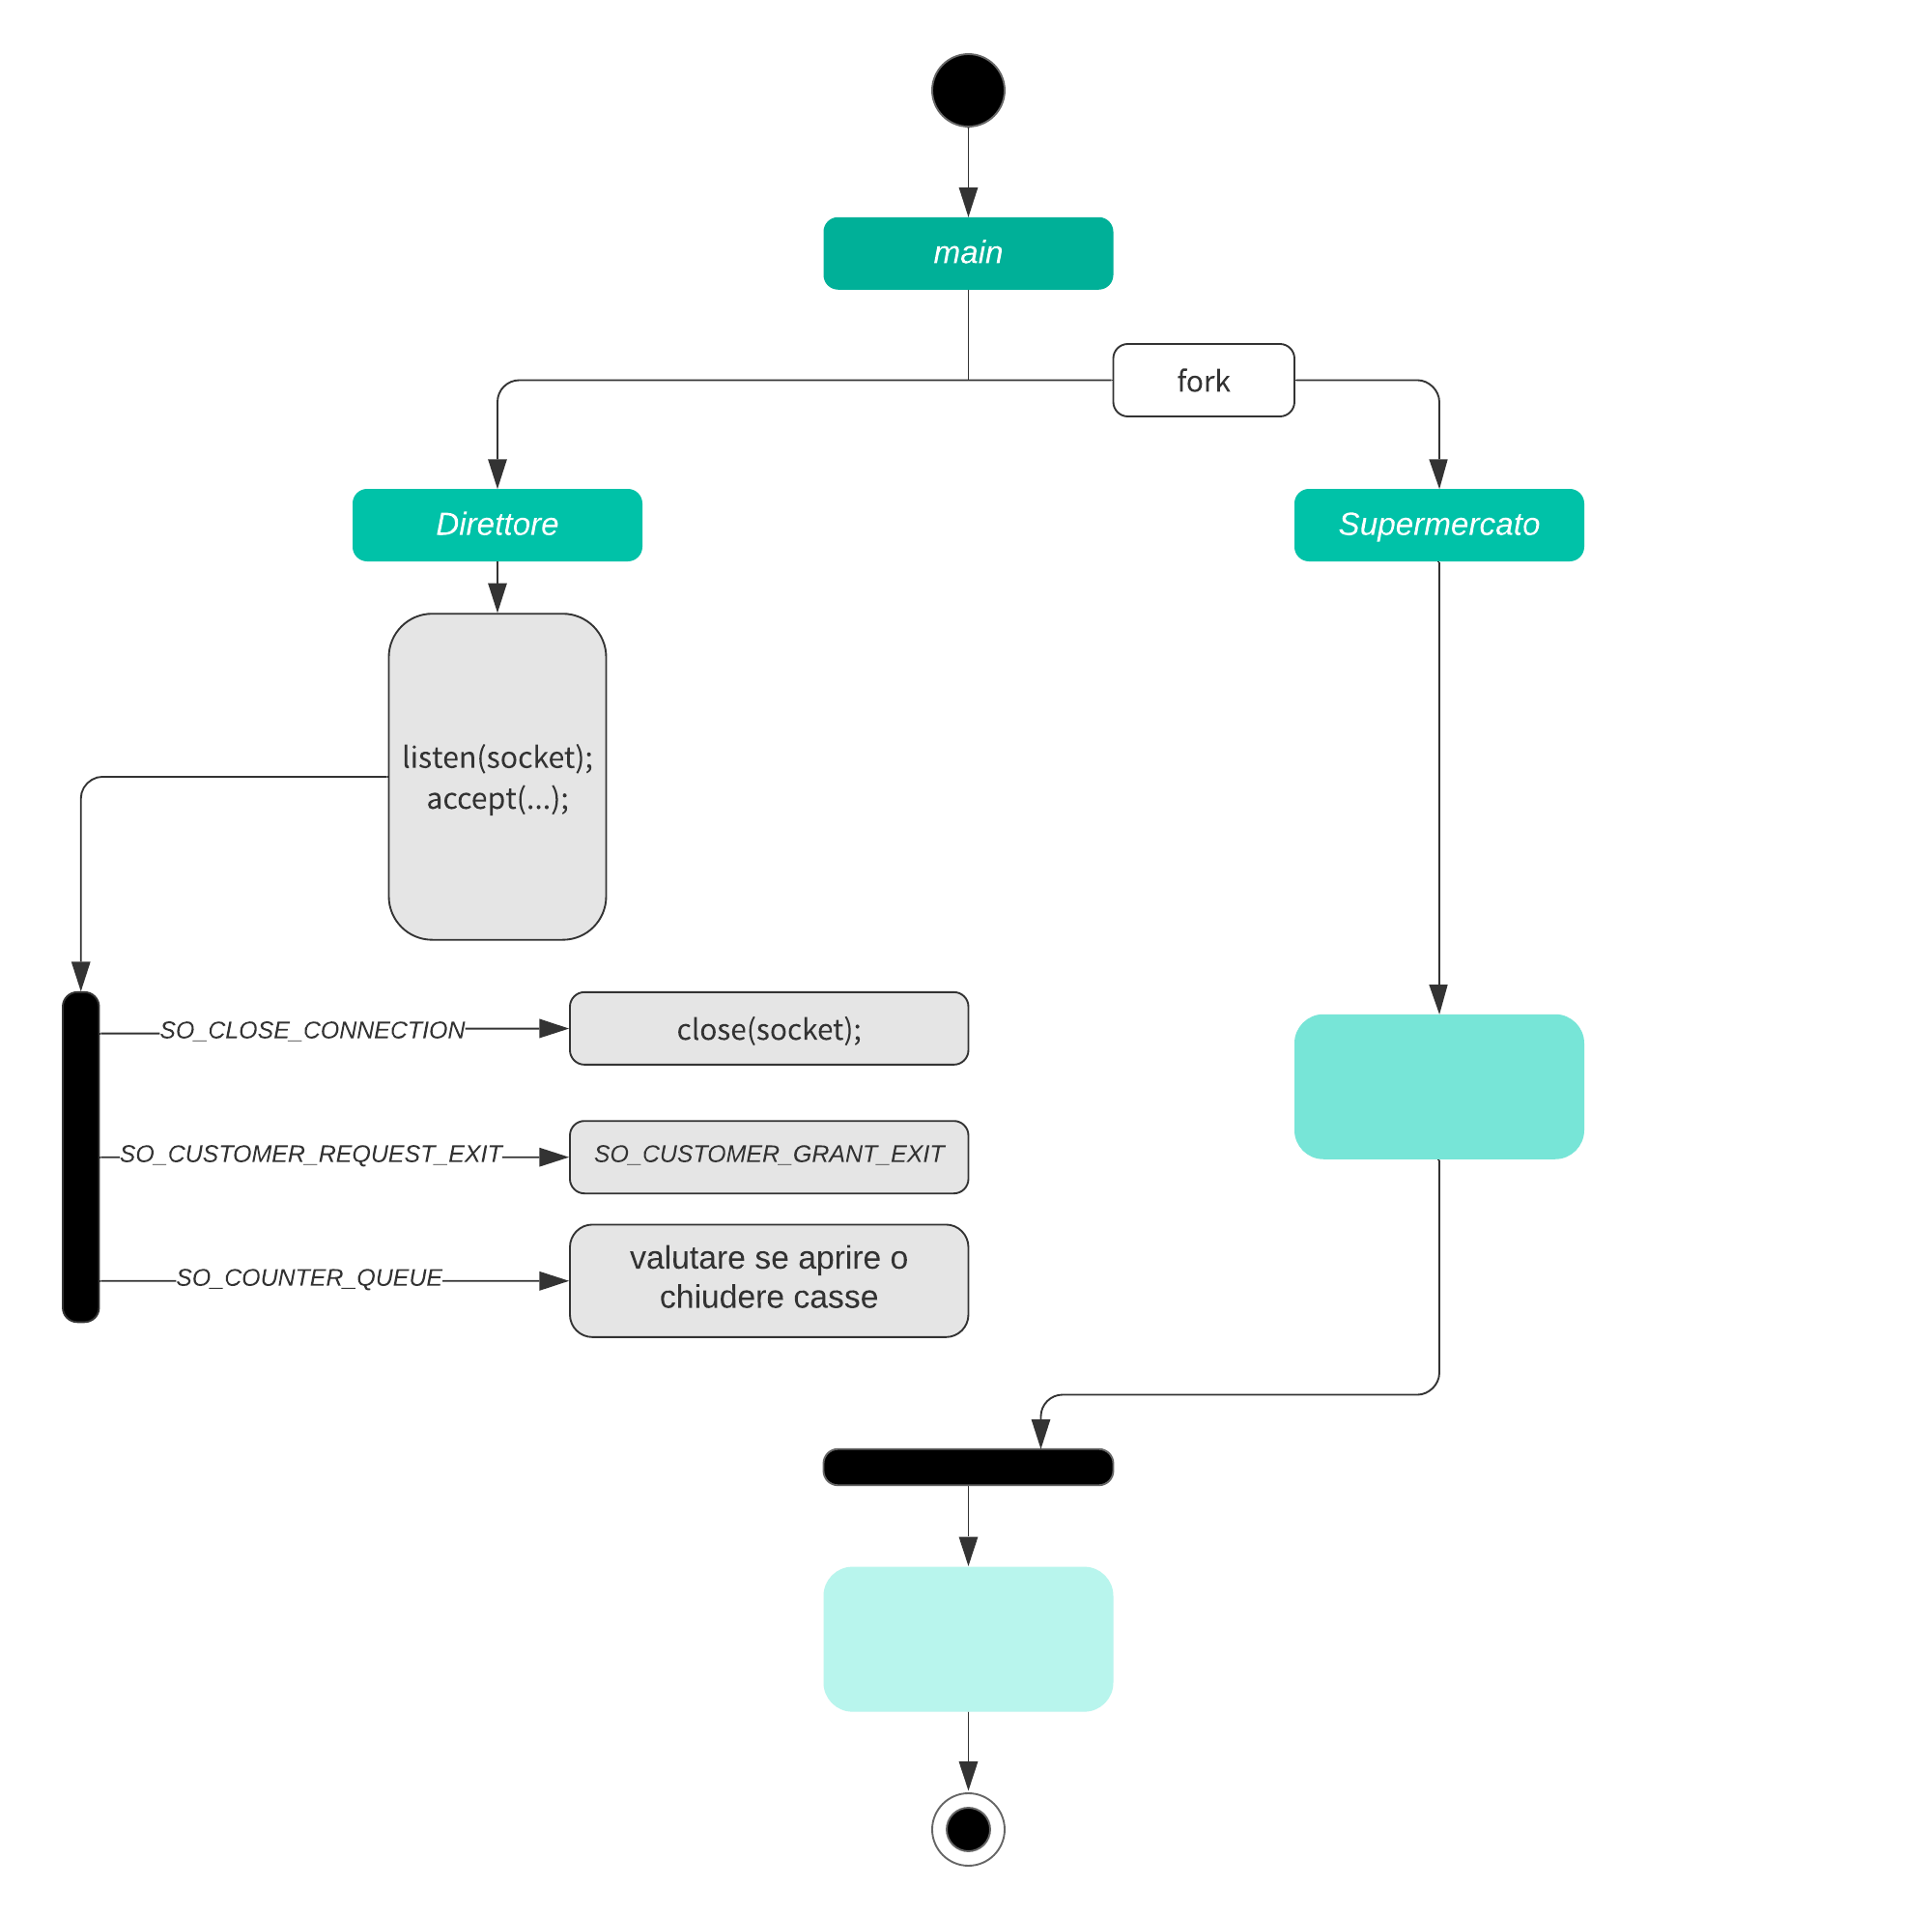
\includegraphics[width=.8\textwidth]{chart}
		\caption{\small Lo schema non è preciso e non rispetta nessuno standard, ma rappresenta una buona approssimazione della struttura del programma}
	\end{center}
\end{figure}

\subsection*{Utility ed Errori}

La gestione degli errori è volutamente molto minimale: poiché la corretta esecuzione del programma richiede il funzionamento di determinate system call, non vi è motivo di tentare di continuare l'esecuzione a seguito di un errore da parte di una di queste. La gestione degli errori si occupa perciò principalmente di stampare informazioni utili al debug e all'individuazione della sorgente del problema.\\
L'unica eccezione riguarda la gestione degli errori legati alla comunicazione via socket, che, nel caso di timeout, esegue qualche tentativo in più prima di comportare il crash.

Di supporto al progetto è stata realizzata una semplice libreria, \lstinline{libllds}, che implementa una queue (utilizzata anche come normale lista), un'hashmap, una read-write lock (implementata secondo lo schema del libro di testo) e offre macro per la gestione degli errori di lock e variabili di condizione. L'implementazione dell'hashmap, in particolare, è volutamente molto semplice, senza ridimensionamento, con un load factor che spesso vale 1 e con una funzione di hash non ottimale. Tuttavia, per l'utilizzo nel progetto, è più che sufficiente e dovrebbe garantire comunque tempi molto veloci.

Tutte le funzioni di utility specifiche al progetto in sé, invece, sono implementate nella cartella \textit{src/utils}. \lstinline{network.c} contiene una funzione per il collegamento al server, con gestione dei timeout. \lstinline{signals.c} implementa una funzione per la registrazione di un handler per i segnali SIGHUP e SIGQUIT e una funzione che invece blocca questi segnali nei thread che non devono gestirli. Ciò fa sì che i segnali siano gestiti dal main thread del supermercato. \lstinline{time.c} implementa alcune funzioni utili ai timer utilizzati nel programma.

\subsection*{Formato File e Script Bash}

Il formato dei file di configurazione e di log è stato scelto in modo da garantire una buona flessibilità e da preferire una certa realisticità rispetto alla pura semplicità di implementazione. Ciò è particolarmente evidente nel formato del file di log, che arriva a supportare anche eventuali commenti. In particolare il formato è il seguente:

\lstinputlisting[language=none]{esempio.log}

Ciò complica un po' il parsing in Bash, che però, grazie alle condizioni in forma \lstinline{if [[ ... ]]}, permettono, differentemente dalle condizioni standard \lstinline{if [ ... ]}, di utilizzare regex e controllare prefissi/suffissi. Ciò sarebbe potuto anche essere implementato utilizzando i \lstinline{case}, che però sarebbero diventati molto disordinati quando utilizzati per grossi blocchi di codice, e perciò sono presenti solo nel caso di brevi istruzioni.\\
L'impaginazione viene effettuata con l'ausilio del comando \lstinline{column}, che però richiede l'utilizzo di un file temporaneo contenente i dati processati dal parser.

\subsection*{Il Direttore}

La logica del direttore è interamente implementata nel file \lstinline{manager.c}. Come prima cosa, viene registrato un handler per i due segnali da gestire. In particolare l'handler modifica il valore di una flag, utilizza una \lstinline{write} (handler-safe), e inoltra il segnale al supermercato mediante una chiamata a \lstinline{kill}. È importante che le System Call non vengano interrotte dai segnali, in particolare l'\lstinline{accept} e la \lstinline{wait}, ma ciò vale anche per le \lstinline{read} sui socket. Per questo viene impostata l'apposita flag SA\_RESTART.

Dopo l'inizializzazione di alcune strutture dati, viene avviato il socket e si attende il collegamento del supermercato. Ogni comunicazione tramite socket viene identificata da un intero iniziale, il cui valore viene definito da alcune macro. In questo caso il collegamento viene identificato dalla costante SO\_SUPERMARKET\_CONNECTION. Il socket viene salvato e mantenuto attivo per comunicare le istruzioni riguardanti l'apertura e la chiusura delle casse.

Viene poi avviato un ciclo di \lstinline{accept}, che si occupa di gestire tutte le comunicazioni in entrata, il vero cuore del processo direttore. Al termine del while le comunicazioni vengono chiuse, si attende la chiusura del supermercato e, dopo aver ripulito la memoria, il processo termina.

Le comunicazioni in entrata possono essere di tre tipi. La più semplice, identificata dalla costante SO\_CLOSE\_CONNECTION, viene inviata dal supermercato al termine della chiusura e serve al direttore per chiudere il socket di listen e interrompere quindi il ciclo di accept. Le comunicazioni identificate da SO\_CUSTOMER\_REQUEST\_EXIT, invece, provengono dai clienti che hanno deciso di non acquistare nessun prodotto e che devono chiedere il permesso di uscire. Viene avviato un thread separato che si occupa di rispondere. Le comunicazioni identificate SO\_COUNTER\_QUEUE contengono i messaggi delle casse riguardo lo stato delle code. Vengono anch'esse gestite da un nuovo thread, che si occupa di aggiornare le informazioni della cassa in un'apposita struttura dati, protetta da lock. A quel punto, prendendo in considerazione solo le informazioni ricevute recentemente dai cassieri, si valuta se modificare il numero di casse aperte o meno.

\subsection*{Il Supermercato}

Anche il supermercato (\lstinline{supermarket.c}) come prima cosa si occupa di registrare l'handler per i segnali, che semplicemente imposta un'apposita flag. In questo caso, tuttavia, è importante che i segnali interrompano le system call e in particolar modo il ciclo di read sul socket di comunicazione con il direttore. È quindi necessario garantire che sia questo il thread che esegue l'handler. A questo scopo, tutti gli altri thread, come prima cosa, chiamano una funzione che blocca i segnali in arrivo.

Il supermercato poi inizializza il logger, le casse, la connessione con il direttore, lancia il thread guardia e avvia il loop di gestione delle casse. Quando questo viene interrotto dal segnale, viene avviato il processo di chiusura del supermercato, diverso per SIGQUIT rispetto a SIGHUP. Nel primo caso, in particolare, come prima cosa vengono chiuse tutte le casse. Questo perché i clienti sanno che, se tutte le casse sono chiuse, devono uscire immediatamente. La funzione \lstinline{guard_close} comunica alla guardia di interrompere il proprio ciclo di creazione di clienti. Questa funzione accetta un parametro che indica se la guardia debba cacciare i clienti fuori dall'edificio o se debba lasciare che questi concludano i propri acquisti. Il \lstinline{pthread_join}, poi, permette alla guardia di attendere che tutti i clienti escano dal supermercato prima di continuare. Se le casse non sono ancora state chiuse, vengono chiuse adesso. Poi si comunica al direttore di chiudere il socket e, in seguito al salvataggio finale dei log, viene liberata la memoria e terminato il processo.

Le strutture dati riguardanti la situazione attuale delle casse, in particolare quelle che indicano il numero di casse aperte, sono protette da una read-write lock, che, poiché i dati vengono continuamente letti da thread diversi, ma scritti solo da quello principale, permette di avere un overhead minimo.

Si è scelto di aprire e chiudere le casse in modo tale che, con K casse operative, le casse aperte siano quelle con id nel range $\left[0,K\right)$. Questo comporta molti vantaggi nello sviluppo, mantenendo compatto sia il codice di apertura/chiusura, sia il codice del cliente che deve scegliere una cassa a cui accodarsi. Ciò tuttavia comporta situazioni non ottimali, come nel caso in cui ad essere chiusa sia la cassa con più clienti in coda. Si ritiene però che, poiché i clienti si ridistribuiscono casualmente sulle altre casse, e poiché questi in ogni caso valutano molto frequentemente se cambiare coda, questo non comporti un grande overhead.

\subsection*{Le Casse}

Le casse, implementate nel file \lstinline{counter.c} sono legate a una struttura dati piuttosto massiccia, di cui però la maggior parte viene utilizzata per memorizzare informazioni ``statistiche'' per il file di log. Degni di nota sono, però, l'id, la coda, lo status, la lock, la variabile di condizione e il timer per la comunicazione con il direttore. Una peculiarità della cassa è che non detiene mai più di una lock alla volta. In particolare, poiché durante il servizio non opera su suoi dati pubblici, può liberare la propria lock prima di ottenere quella del cliente, evitando quindi la possibilità di deadlock. Alcune particolari race condition sono comunque possibili, ma possono essere riconosciute ed evitate senza l'utilizzo di lock doppie (se non per quanto riguarda il thread cliente, che si esaminerà più avanti).

Il ciclo principale della cassa viene eseguito finché lo status è diverso da CLOSED. Al suo interno vi è un ulteriore while che, nel caso in cui nessun cliente sia in coda, attende sulla variabile di condizione. Altrimenti, viene come prima cosa controllato se la cassa sia in stato CLOSING e quindi debba essere iniziata la procedura di chiusura, oppure se sia il caso di servire il prossimo cliente in coda. La funzione \lstinline{counter_close}, dopo aver gestito le statistiche da loggare, comunica a tutti i clienti in coda che devono cambiare cassa. Per fare ciò li rimuove dalla loro coda corrente, dopo aver verificato che non l'abbiano cambiata nel frattempo. I clienti si renderanno conto da soli a breve di non essere più in nessuna coda e ne cercheranno un'altra. Il servizio del cliente, invece, viene eseguito in maniera semplice, con l'aggiornamento di alcune variabili e un'opportuna attesa.

Tuttavia la cassa deve anche tenere conto di quando sia il momento di comunicare al direttore il numero di clienti in coda. A tale scopo vengono adottate due diverse strategie. Nel caso della wait sulla variabile di condizione, si utilizza una chiamata a \lstinline{pthread_cond_timedwait}, che permette di risvegliarsi dopo un determinato intervallo di tempo per poi chiamare la funzione \lstinline{counter_notify_manager}. Nel caso dell'attesa per il servizio del cliente, invece, si utilizza una chiamata a \lstinline{nanosleep}. Un wrapper di questa funzione si occupa di calcolare se e come spezzare l'attesa in modo da permettere una chiamata a \lstinline{counter_notify_manager} nel mezzo.

La funzione \lstinline{counter_notify_manager}, che, per evitare situazioni di stallo, deve essere chiamata senza detenere nessuna lock, stabilisce una comunicazione con il direttore, comunica il numero di casse aperte e il numero di clienti in coda alla cassa corrente e vi associa un timestamp. Questo è indispensabile affinché il direttore possa prendere decisioni basandosi solo su informazioni recenti.

\subsection*{I Clienti}

Il thread clienti è implementato in \lstinline{customer.c} ed è anch'esso associato a un'opportuna struttura dati. Dopo un'attesa iniziale, legata all'acquisto dei prodotti, se il loro numero è nullo, il cliente chiede il permesso al direttore di uscire e, dopo averlo ricevuto, comincia direttamente il suo processo di terminazione. Altrimenti, comincia la gestione delle code. In un ciclo while, eseguito finché lo status vale QUEUE, il cliente sceglie una cassa a cui accodarsi e attende finché o non viene servito oppure non esce dalla coda. Il cliente può uscire dalla coda per due ragioni, o perché la cassa è stata chiusa, oppure perché, periodicamente, a seguito di un'attesa, il cliente valuta se cambiare coda o meno. L'algoritmo per la decisione del cambio coda tiene conto del numero di persone alla cassa corrente e di un livello di pazienza personale.
Quando il while esterno termina, significa che il cliente sta venendo servito, ed è quindi il momento di attendere su una variabile condizione che il cassiere termini il suo lavoro.

Il processo di terminazione di un cliente include la comunicazione alla guardia del fatto che si stia uscendo e la stampa dei propri dati su file di log.

Le attese del cliente sono anch'esse implementate tramite \lstinline{nanosleep}. Tuttavia, in questo caso, bisogna gestire un evento particolare. Quando il supermercato riceve un segnale SIGQUIT, tutti i clienti devono interrompere le loro attese e uscire immediatamente. A tale scopo, la guardia invia un segnale SIGUSR1 a tutti i thread clienti, con l'obiettivo di interrompere la System Call di attesa. È lecito chiedersi se questa sia la strategia migliore, o se invece sia meglio utilizzare una condition variable unitamente a \lstinline{pthread_cond_timedwait}, similarmente a ciò che si è fatto con le casse, in modo che la guardia possa più semplicemente chiamare una \lstinline{pthread_cond_signal}. Ciò eviterebbe anche la necessità di registrare un handler vuoto per ogni cliente. Tuttavia questa strategia, oltre a necessitare di una più complessa gestione nel caso di spurious wakeup, si rivela anche impossibile. Il cliente, infatti, decide se cambiare coda ogni S millisecondi. Questo valore è piuttosto piccolo (30 nel caso dei test) e ciò comporta che, nella maggior parte dei casi, la wait venga subito interrotta e la lock non venga mai liberata. Se la lock non può essere liberata, la cassa non può servire il cliente, e il programma non termina. Per verificare la natura del problema, si è provato a utilizzare tempi maggiori (300ms) e si è visto che effettivamente le casse erano in grado di servire i clienti e il programma eseguiva normalmente.

La principale causa di questa problematica è dovuta al fatto che, mentre la funzione \lstinline{nanosleep} si aspetta un numero di nanosecondi da attendere, la funzione \lstinline{pthread_cond_timedwait} richiede l'indicazione del tempo assoluto fino a cui aspettare. Evidentemente il calcolo di questo tempo, comprendente la chiamata a un paio di funzioni, unitamente al tempo impiegato dallo scheduler dei thread, fa sì che, per intervalli così brevi, il tempo assoluto sia già stato raggiunto (o quasi) al momento della chiamata alla wait.

Il cliente, differentemente dalla cassa, necessita dell'utilizzo di (almeno) due lock in contemporanea, in particolare la propria e quella della cassa a cui vuole accodarsi o dalla cui coda vuole uscire. Poiché, come si è visto, la cassa non detiene mai le due lock nello stesso momento, non si possono verificare stalli dovuti all'ordine di lock. Tuttavia, esiste la remota possibilità che si verifichino alcune race condition. Si tratta, però, di situazioni semplici che possono comunque essere evitate. Un esempio è la serie di istruzioni \textit{1. rimuovere un cliente dalla coda; 2. sbloccare la cassa; 3. bloccare il cliente} proprie della cassa, e le istruzioni \textit{A. decidere di cambiare coda; B. bloccare la cassa; C. uscire dalla coda} proprie del cliente. Se queste vengono eseguite nell'ordine \textit{1,2,A,B,C,3}, la cassa si ritroverebbe a servire un cliente che fa parte di un'altra coda. Tuttavia, si può modificare l'istruzione \textit{C}, affinché il cliente esca dalla coda solo dopo aver controllato di farne ancora parte. Ciò è reso ancora più semplice dall'interfaccia della struttura \lstinline{queue}, che, al momento della rimozione, ritorna NULL in caso l'elemento non faccia parte della coda. Questo controllo si trova nella funzione \lstinline{customer_consider_queue_change}.

\subsection*{La Guardia}

Come anticipato, la guardia si occupa della gestione dei clienti in entrata e in uscita. Per far ciò, si avvale di un'hashmap contenente i \lstinline{pthread_t} di ogni cliente. Dopo la sua inizializzazione, la guardia entra in un loop il cui scopo è quello di attendere (mediante una variabile di condizione) che il numero di clienti scenda sotto C - E, e, nel momento in cui ciò accade, di creare i nuovi clienti con annesso thread. Quando il supermercato deve chiudere, se ciò avviene in seguito a un segnale SIGQUIT, la guardia preleva i \lstinline{pthread_t} dall'hashmap e, mediante la chiamata a \lstinline{pthread_kill}, invia un segnale SIGUSR1 a tutti i clienti, con lo scopo analizzato sopra. Sempre mediante una variabile di condizione, la guardia aspetta che tutti i clienti escano. Quando un cliente esce, infatti, aggiorna gli opportuni contatori, si rimuove dall'hashmap e chiama la \lstinline{pthread_cond_signal}.

\end{document}
